\section{Related Work}

\label{sec:related-work}
\begin{figure*}[t]
\centering
	\makebox[0.4\textwidth][c]{
		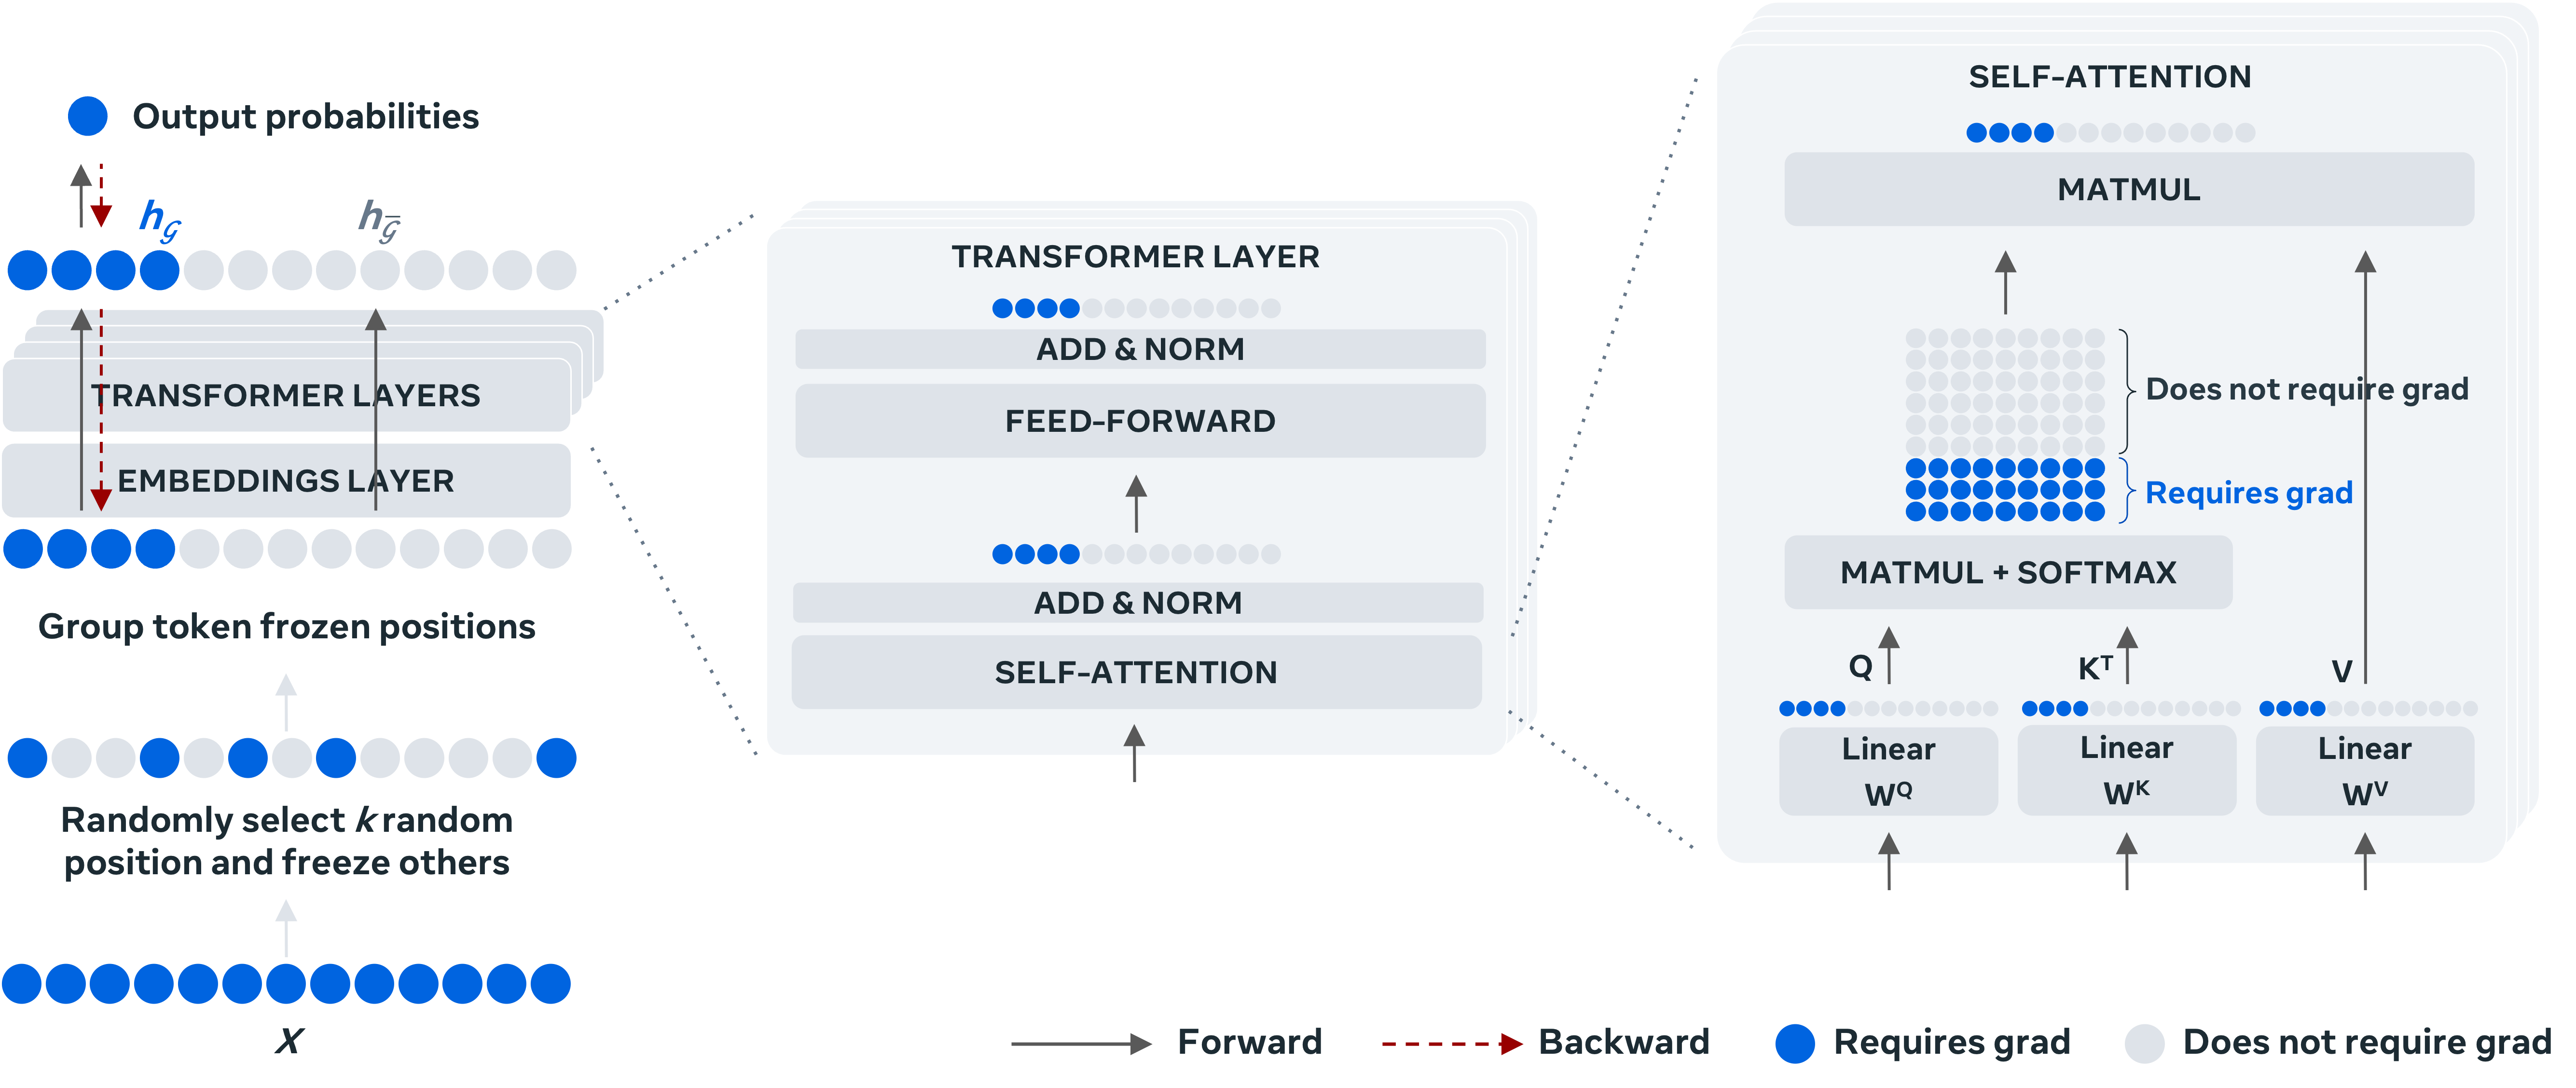
\includegraphics[width=1.0\textwidth]{figures/method_overview_3.png}
}
\caption{\method achieves memory-efficient fine-tuning of transformers via token selection.
		During the backward pass, we compute the gradient for only a subset of $k$ input tokens, while the others are frozen (in \textcolor{gray}{gray} in the figure).
		During the forward pass, all input positions are used, but only a subset of the activations is cached~in~memory (in \textcolor{blue}{blue} in the figure).
		\method is applicable to various transformer-based models, as well as different language modeling tasks, as our experiments with \textsc{Bert}~\citep{devlin_19} and Llama~\citep{touvron_23} show.
}
\label{fig:method}
\end{figure*}

\subsection{Parameter-Efficient Fine-Tuning (PEFT)}
PEFT methods, which aim to limit the computing resources for fine-tuning LLMs, 
can be divided into four categories~\citep{DBLP:journals/corr/abs-2403-14608,DBLP:journals/corr/abs-2312-12148}.

\paragraph{Selective PEFT} methods update only a subset of the backbone model parameters
using weight masking strategies, such as
learnable binary masking~\citep{DBLP:conf/acl/GuoRK20} and parameter importance estimation using Fisher information~\citep{DBLP:conf/nips/SungNR21,DBLP:conf/emnlp/DasZS0Z23}. Other selective PEFT methods focus on updating specific modules,
e.g., the cross-attention layers~\citep{DBLP:conf/emnlp/Gheini0M21} and the bias terms~\citep{zaken_22,DBLP:conf/acl/LawtonKTGS23}.  

\paragraph{Additive PEFT} methods add a few parameters to the frozen pre-trained model, 
and fine-tune only the added parameters. E.g., adapters inject small layers within the transformer block,
either sequentially after its sublayers~\citep{DBLP:conf/icml/HoulsbyGJMLGAG19,DBLP:conf/eacl/PfeifferKRCG21}, or as a side network running in parallel to the sublayers~\citep{DBLP:conf/iclr/HeZMBN22,DBLP:conf/emnlp/ZhuFZWL21}.
Alternatively, soft prompt-based approaches~\citep{DBLP:conf/acl/LiL20,qin_21,liu_21} 
prepend continuous learnable vectors to the input of a frozen model and tune them for each~task.

\paragraph{Reparameterized PEFT} methods perform low-rank transformation,
utilizing the low intrinsic dimension of LLMs~\citep{DBLP:conf/acl/AghajanyanGZ20}.  LoRA~\citep{hu_22} is the most representative approach, 
where an update to the model weights is captured via its low-rank decomposition.
Several studies followed to improve LoRA, e.g., 
to support dynamic rank selection~\citep{DBLP:conf/eacl/ValipourRKG23,DBLP:conf/iclr/ZhangCBH0CZ23}, and to address overfitting~\citep{DBLP:journals/corr/abs-2404-09610} and overconfidence~\citep{DBLP:conf/iclr/YangRWA24}.  

\paragraph{Hybrid PEFT} methods aim to combine different PEFT approaches, e.g.,
adapters, prefix-tuning, and LoRA.
The design space of combinations of PEFT methods has been explored
either manually~\citep{DBLP:conf/iclr/HeZMBN22,DBLP:conf/acl/MaoMHAM0YK22}, or automatically, e.g., by leveraging neural architecture search methods~\citep{DBLP:journals/corr/abs-2206-04673,DBLP:journals/tacl/ZhouWVK24}. 

\paragraph{\kern-0.3em}
While the above PEFT methods effectively improve parameter efficiency,
they may still incur significant memory overhead during fine-tuning~\citep{sung2022lst,DBLP:conf/emnlp/JinZZ23}.
The proposed \method can be combined with these PEFT methods,
enabling them to achieve both parameter and memory efficiency,
as \Cref{sec:exp:medium,sec:exp:large} show.





\subsection{Memory-Efficient Fine-Tuning}

There exist several techniques that can be used to improve the memory efficiency in fine-tuning LLMs,
which we organize into four groups.


\paragraph{Memory-Efficient PEFT.}
Some PEFT methods aim to achieve memory and parameter efficiency simultaneously.
Side tuning methods~\citep{zhang_20, sung2022lst}
introduce small learnable side networks separated from the backbone model, and
channel backpropagation only through the side networks, 
thereby reducing the memory requirements for gradients and intermediate activations.
By utilizing the reversible model, 
MEFT~\cite{DBLP:conf/nips/LiaoTM23} avoids the need to cache intermediate activations in the forward pass.
LoRA-FA~\citep{DBLP:journals/corr/abs-2308-03303} improves LoRA
by addressing its high memory usage for input activations
via freezing LoRA's down-projection weights.


\paragraph{Gradient Checkpointing}~\citep{DBLP:journals/corr/ChenXZG16,DBLP:conf/nips/GruslysMDLG16}
reduces the memory requirement for model training
by storing only a subset of intermediate activations in the forward pass, and recomputing the others during the backward pass.



\paragraph{Quantization} is a compression technique that reduces the number of bits for storing numerical values. 
With quantization, parameters are represented with lower-precision data types~\citep{dettmers_22, dettmers_23, liu_23},
leading to memory reduction in both fine-tuning and inference.

\paragraph{Approximate Gradient Methods} reduce the memory usage
by avoiding the exact gradient computation involved with full fine-tuning, and 
instead using an approximate estimate of the gradient for weight updates.
To this end, a few methods employ low-rank factorization,
where they reduce memory cost by utilizing 
the low-rank structure of the gradients~\citep{zhao2024galore} or the second-order statistics~\citep{DBLP:conf/icml/ShazeerS18}. Alternatively, MeZO~\citep{DBLP:conf/nips/MalladiGNDL0A23} 
approximates the gradient using only forward passes,
building upon the zeroth-order optimization technique~\cite{Spall1992MultivariateSA}.



\paragraph{\kern-0.3em}
The proposed \method can be considered an approximate gradient method, 
as its token-selective fine-tuning strategy leads to an approximation of the full gradient,
which is a completely new direction investigated to improve memory efficiency in fine-tuning.
Also, being complementary to prior methods, 
\method can be combined with them, resulting in further memory reduction.








